%% 美赛模板:正文部分

\documentclass[12pt]{article}  % 官方要求字号不小于 12 号,此处选择 12 号字体

% 本模板不需要填写年份,以当前电脑时间自动生成
% 请在以下的方括号中填写队伍控制号
\usepackage[2506135]{easymcm}  % 载入 EasyMCM 模板文件
\problem{C}  % 请在此处填写题号
\usepackage{mathptmx}  % 这是 Times 字体,中规中矩 
%\usepackage{mathpazo}  % 这是 COMAP 官方杂志采用的更好看的 Palatino 字体,可替代以上的 mathptmx 宏包
\usepackage{amsmath}
\usepackage{tabularray}
%拉取的一些宏包
\usepackage{graphicx} 
%\usepackage{pdfpages}
\usepackage{longtable}
%\usepackage{tabu}
\usepackage{threeparttable} %支持在表格中使用 \tnote 命令添加脚注,并自动编号
\usepackage{listings} %在文档中插入代码
%\usepackage{paralist}%创建紧凑的列表,节省垂直空间
%\usepackage{setspace} %调整文档的行间距
%\usepackage{booktabs}%用于创建更美观的表格,提供了高质量的表格线条命令,如 \toprule、\midrule 和 \bottomrule
%\usepackage{makecell} %创建多行单元格,支持复杂的表格布局
\usepackage{amssymb} %提供了额外的数学符号,通常与 amsmath 宏包一起使用
\usepackage{appendix} %管理附录部分,自动处理附录的编号和格式
\newcommand{\upcite}[1]{\textsuperscript{\textsuperscript{\cite{#1}}}}


\title{Together, Individuals Make a Difference}  % 标题

% 如需要修改题头(默认为 MCM/ICM),请使用以下命令(此处修改为 MCM)
%\renewcommand{\contest}{MCM}

% 文档开始
\newtheorem{keywords}{Keywords}
\begin{document}

% 此处填写摘要内容
\begin{abstract}
    Here is the abstract of your paper.

    Firstly, that is ...

    Secondly, that is ...

    Finally, that is ...

$F(\omega) = \int_{-\infty}^{\infty} f(t) e^{-i \omega t} \, dt$


$f(t) = \frac{1}{2\pi} \int_{-\infty}^{\infty} F(\omega) e^{i \omega t} \, d\omega$

    % 美赛论文中无需注明关键字。若您一定要使用,
    % 请将以下两行的注释号 '%' 去除,以使其生效
    % \vspace{5pt}
    % \textbf{Keywords}: MATLAB, mathematics, LaTeX.
    
    
    \textbf{PCA}\\
    \%\\
    % 关键字Keywords
    \vspace{5pt}
    \textbf{Keywords}: \textbf{ A, B, C,  }
    
	
\end{abstract}

\maketitle  % 生成 Summary Sheet
\tableofcontents  % 生成目录


% 正文开始
\section{Introduction}
\subsection{Problem Background}


\subsection{Restatement of Problem}
A literatrue\cite{1} say something about this problem ...
There is a conception named "momentum" in tennis, which has a great impact on players' performance. It is a generalization of the influence in manifold aspects like mental stress and residual energy. So the fluctuation of momentum is the most probable factor that reveals the trend of match. However,the momentum is not easy to be quantified for it includes many subjective indicators, and there are few models that can be directly used, so we decide to cut in the following questions from statistical analysis and data procession:

\begin{itemize}
	\setlength{\parsep}{0ex} %段落间距
	\setlength{\topsep}{2ex} %列表到上下文的垂直距离
	\setlength{\itemsep}{1ex} %条目间距
	\item Develop a model that captures the flow of play as points occur and apply it to one or more of the matches. Your model should identify which player is performing better at a given time in the match, as well as how much better they are performing. Provide a visualization based on your model to depict the match flow. \textit{Note: in tennis, the player serving has a much higher probability of winning the point/game. You may wish to factor this into your model in some way.}
	\item A tennis coach is skeptical that “momentum” plays any role in the match. Instead, he postulates that swings in play and runs of success by one player are random. Use your model/metric to assess this claim.
	\item Coaches would love to know if there are indicators that can help determine when the flow of play is about to change from favoring one player to the other.
	\begin{itemize}
		\item[1)]
		Using the data provided for at least one match, develop a model that predicts these swings in the match. What factors seem most related (if any)?
	\end{itemize}
	\begin{itemize}
		\item[2)]
		Given the differential in past match “momentum” swings how do you advise a player going into a new match against a different player?
	\end{itemize}
	\item Test the model you developed on one or more of the other matches. How well do you predict the swings in the match? If the model performs poorly at times, can you identify any factors that might need to be included in future models? How generalizable is your model to other matches (such as Women’s matches), tournaments, court surfaces, and other sports such as table tennis.
	\item Produce a report of no more than 25 pages with your findings and include a one- to two-page memo summarizing your results with advice for coaches on the role of“momentum”, and how to prepare players to respond to events that impact the flow of play during a tennis match.
\end{itemize}

\subsection{Our work}
We do such things ...




%图片示例(water.png)
%\begin{figure}[htbp]
%	\centering
%	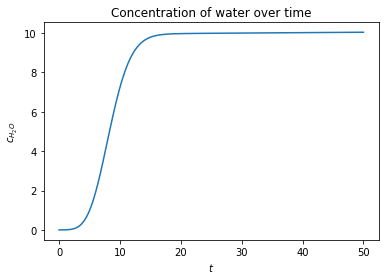
\includegraphics[width=.8\textwidth]{water.png}
%	\caption{The result of Model 2}\label{fig:result}
%\end{figure}
\begin{enumerate}[\bfseries 1.]
    \item We do ...
    \item We do ...
    \item We do ...
\end{enumerate}
\section{Question Preparation}
\subsection{Assumptions}


\subsection{Notations}

The primary notations used in this paper are listed in Table \ref{tb:notation}.

% 三线表示例
\begin{table}[!htbp]
\begin{center}
\caption{Notations}
\begin{tabular}{cl}
	\toprule
	\multicolumn{1}{m{3cm}}{\centering Symbol}
	&\multicolumn{1}{m{8cm}}{\centering Definition}\\
	\midrule
	$C_{i}$&the first one\\
	$S_{i}$&the second one\\
	$G$&the second one\\
	$V$&the second one\\
	$B$&the second one\\
	$M$&the second one\\
	$A$&the second one\\
	$D$&the second one\\
	$E$&the second one\\
%	$\alpha$ &the last one\\
    $\gamma$&Sport Advantagen Coefficient\\
  	$ m_{c_{i}}$ &the second one\\
	$ m_{c_{i} s_{j}}$ &the second one\\
    $g_{i}$&the second one\\
    $\xi$&The Probability of First Medal\\
	\bottomrule
\end{tabular}\label{tb:notation}
\end{center}
\end{table}

\section{Data Preprocessing}
\subsection{Basic Data Preprocessing}

$$G_{i} \cap G_{j}=\emptyset, \bigcup_{i=1}^{5} G_{i}=X$$


\begin{figure}[htbp]
	\centering
	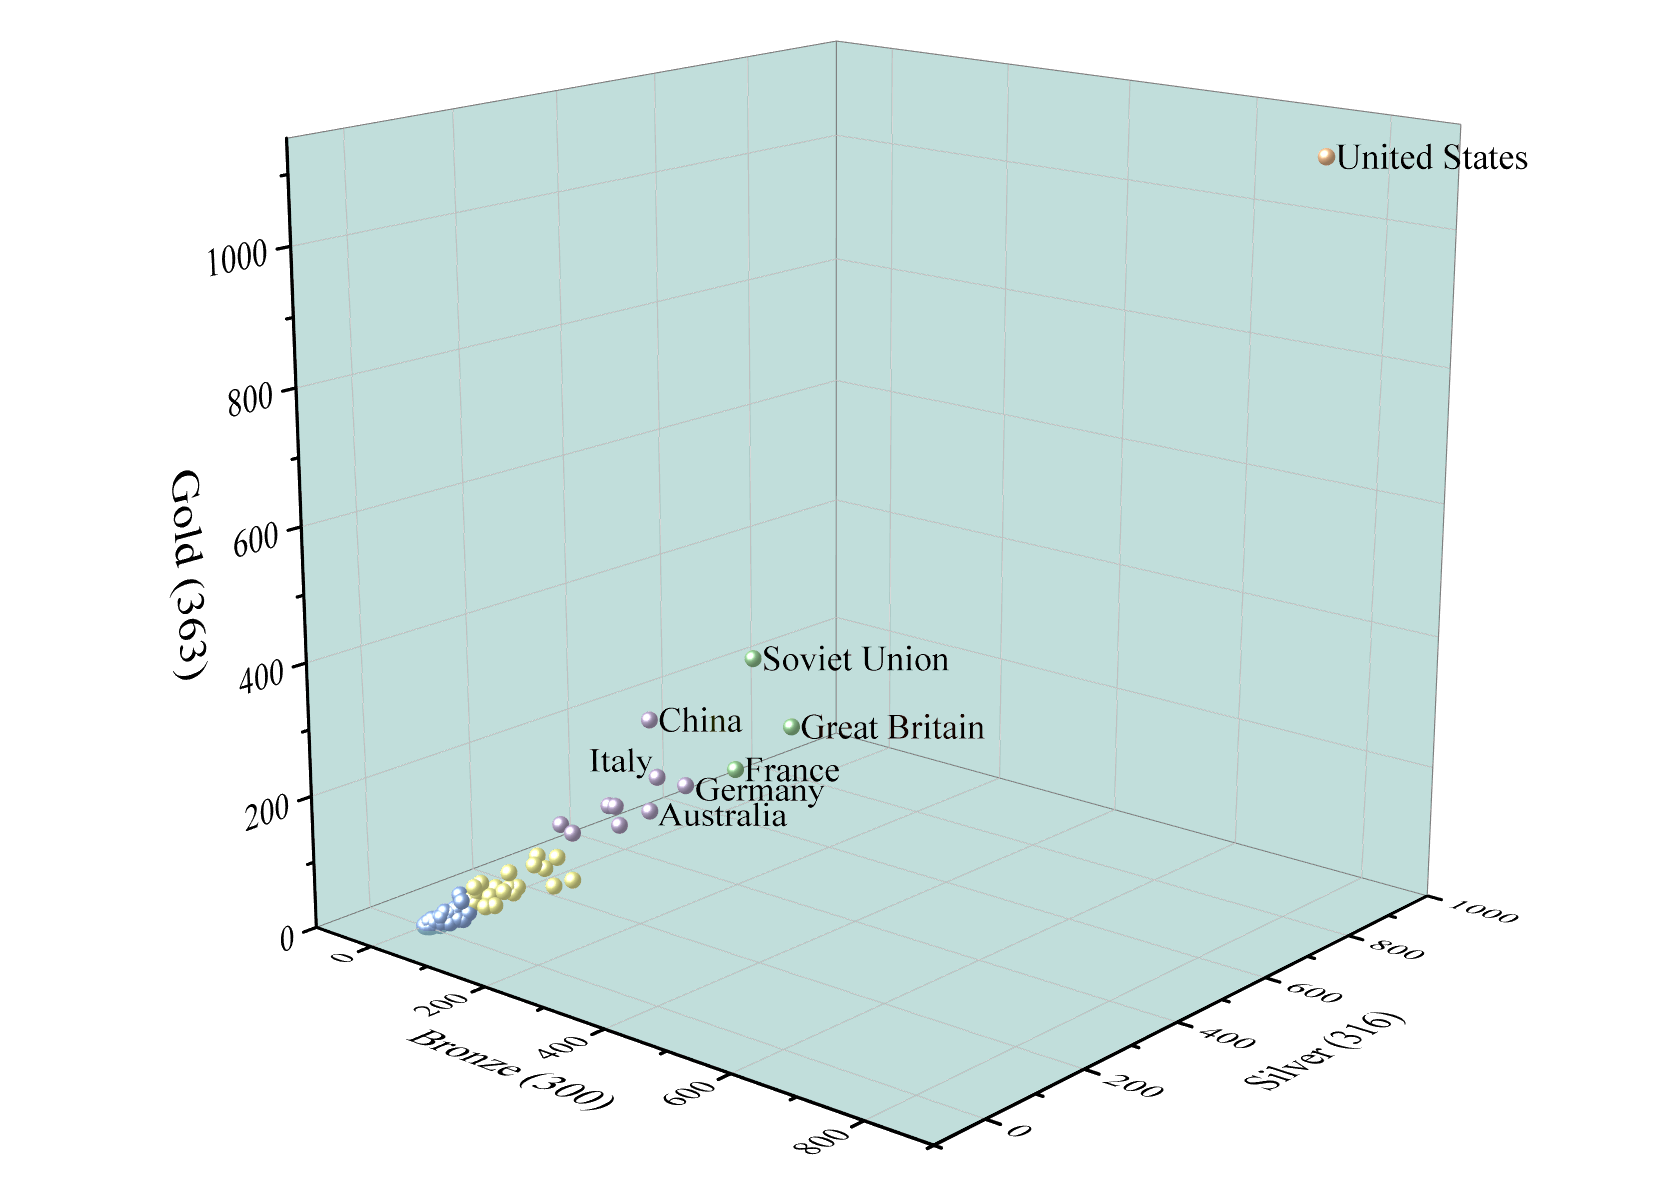
\includegraphics[width=12cm]{img/Level1.png}
	\caption{Scatter plot of national level classification (based on Kmeans++clustering algorithm)}
	\label{fig:aa}
\end{figure}

\begin{figure}[htbp]
	\centering
	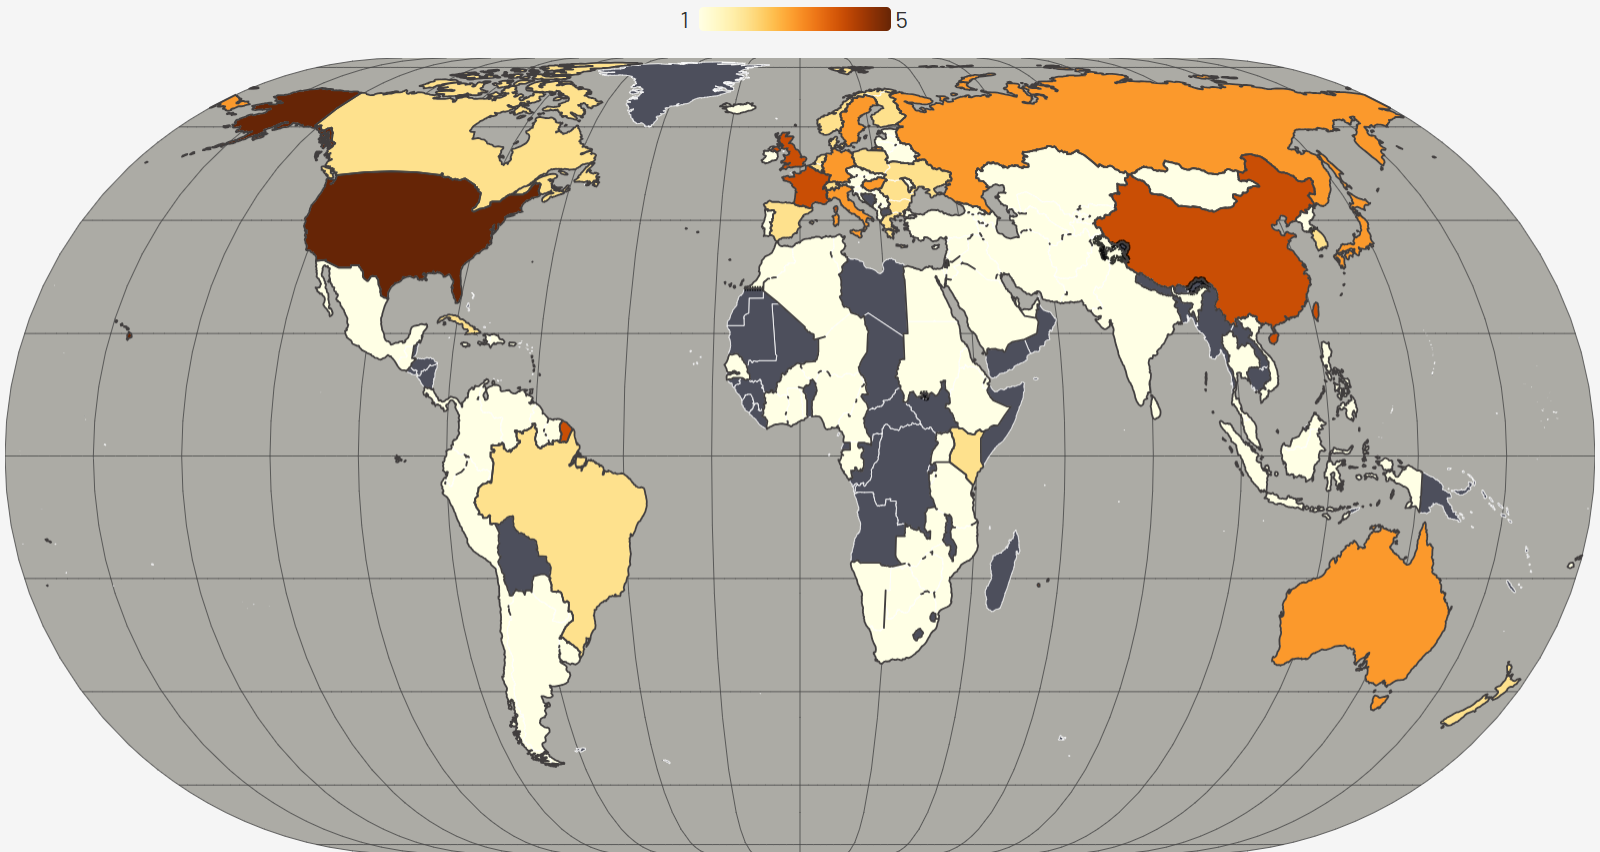
\includegraphics[width=12cm]{img/Level2.png}
	\caption{aa}
	\label{fig:aa}
\end{figure}









\subsection{Data Mining}
\subsubsection{Athlete Service Status}


\begin{figure}[htbp]
	\centering
	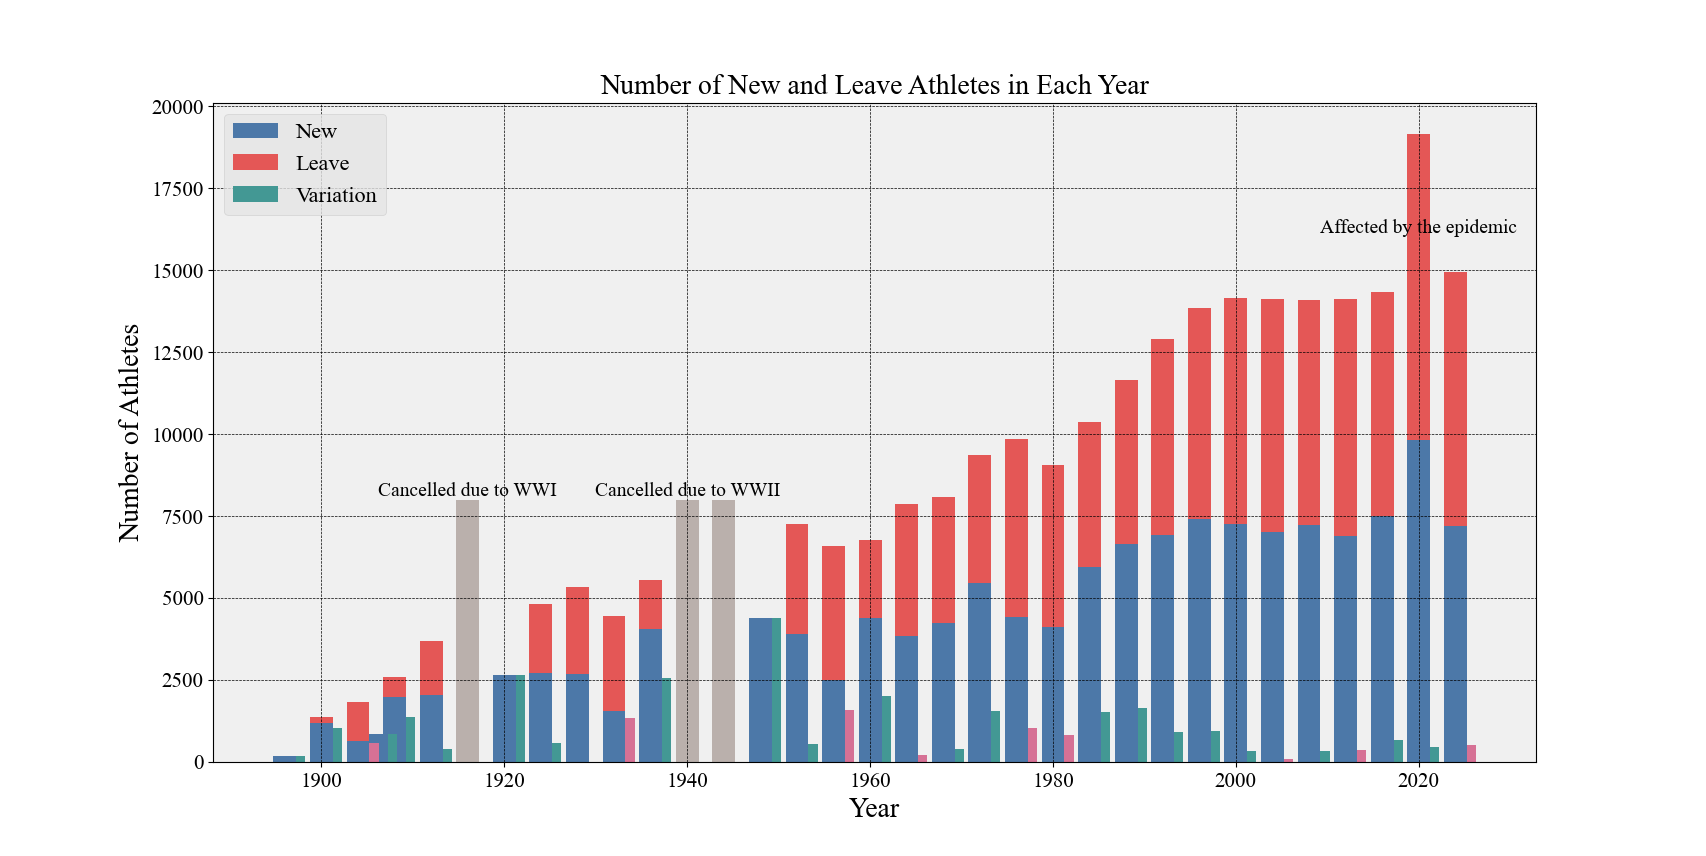
\includegraphics[width=12cm]{img/Number.png}
	\caption{Number of New and Leave Athletes in Each Year}
	\label{fig:aa}
\end{figure}

% 子图(多图并列)示例,更多用法请参考 subfigure 宏包文档
% 如果您只希望几张图并列,不需要额外的 caption,那么在 figure 环境中
% 连续插入总宽度不超过 \textwidth 的多个 \includegraphics 命令即可
\begin{figure}[htbp]
	\centering
	\begin{subfigure}[b]{.55\textwidth}
		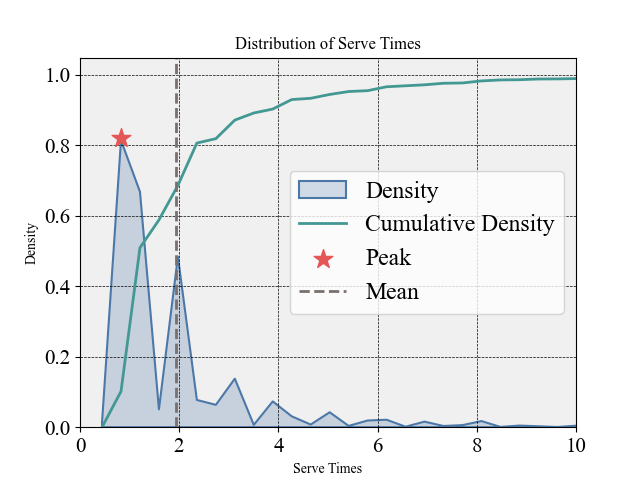
\includegraphics[width=\textwidth]{img/Times.png}
		\caption{Distribution of Serve Times}\label{subfig:left}
	\end{subfigure}
	\begin{subfigure}[b]{.4\textwidth}
		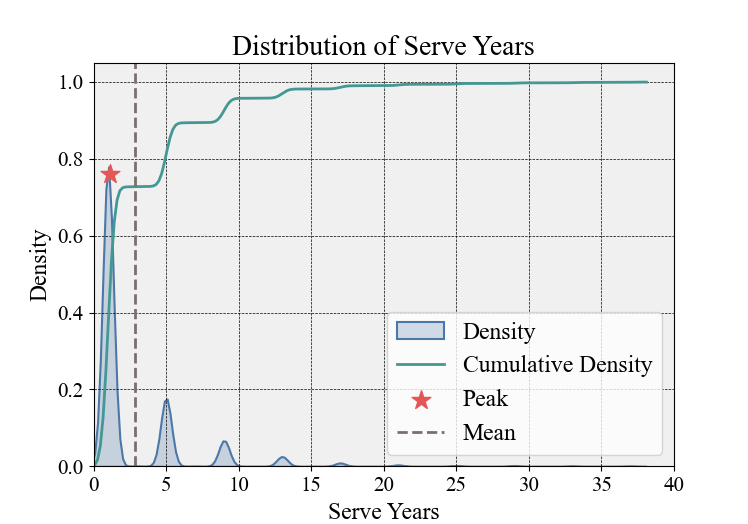
\includegraphics[width=\textwidth]{img/Years.png}
		\caption{Distribution of Serve Years}\label{subfig:right}
	\end{subfigure}
	\caption{Two images}\label{fig:subfigures}
\end{figure}

\subsubsection{Distribution of Countries' Strength Sports}


\begin{figure}[htbp]
	\centering
	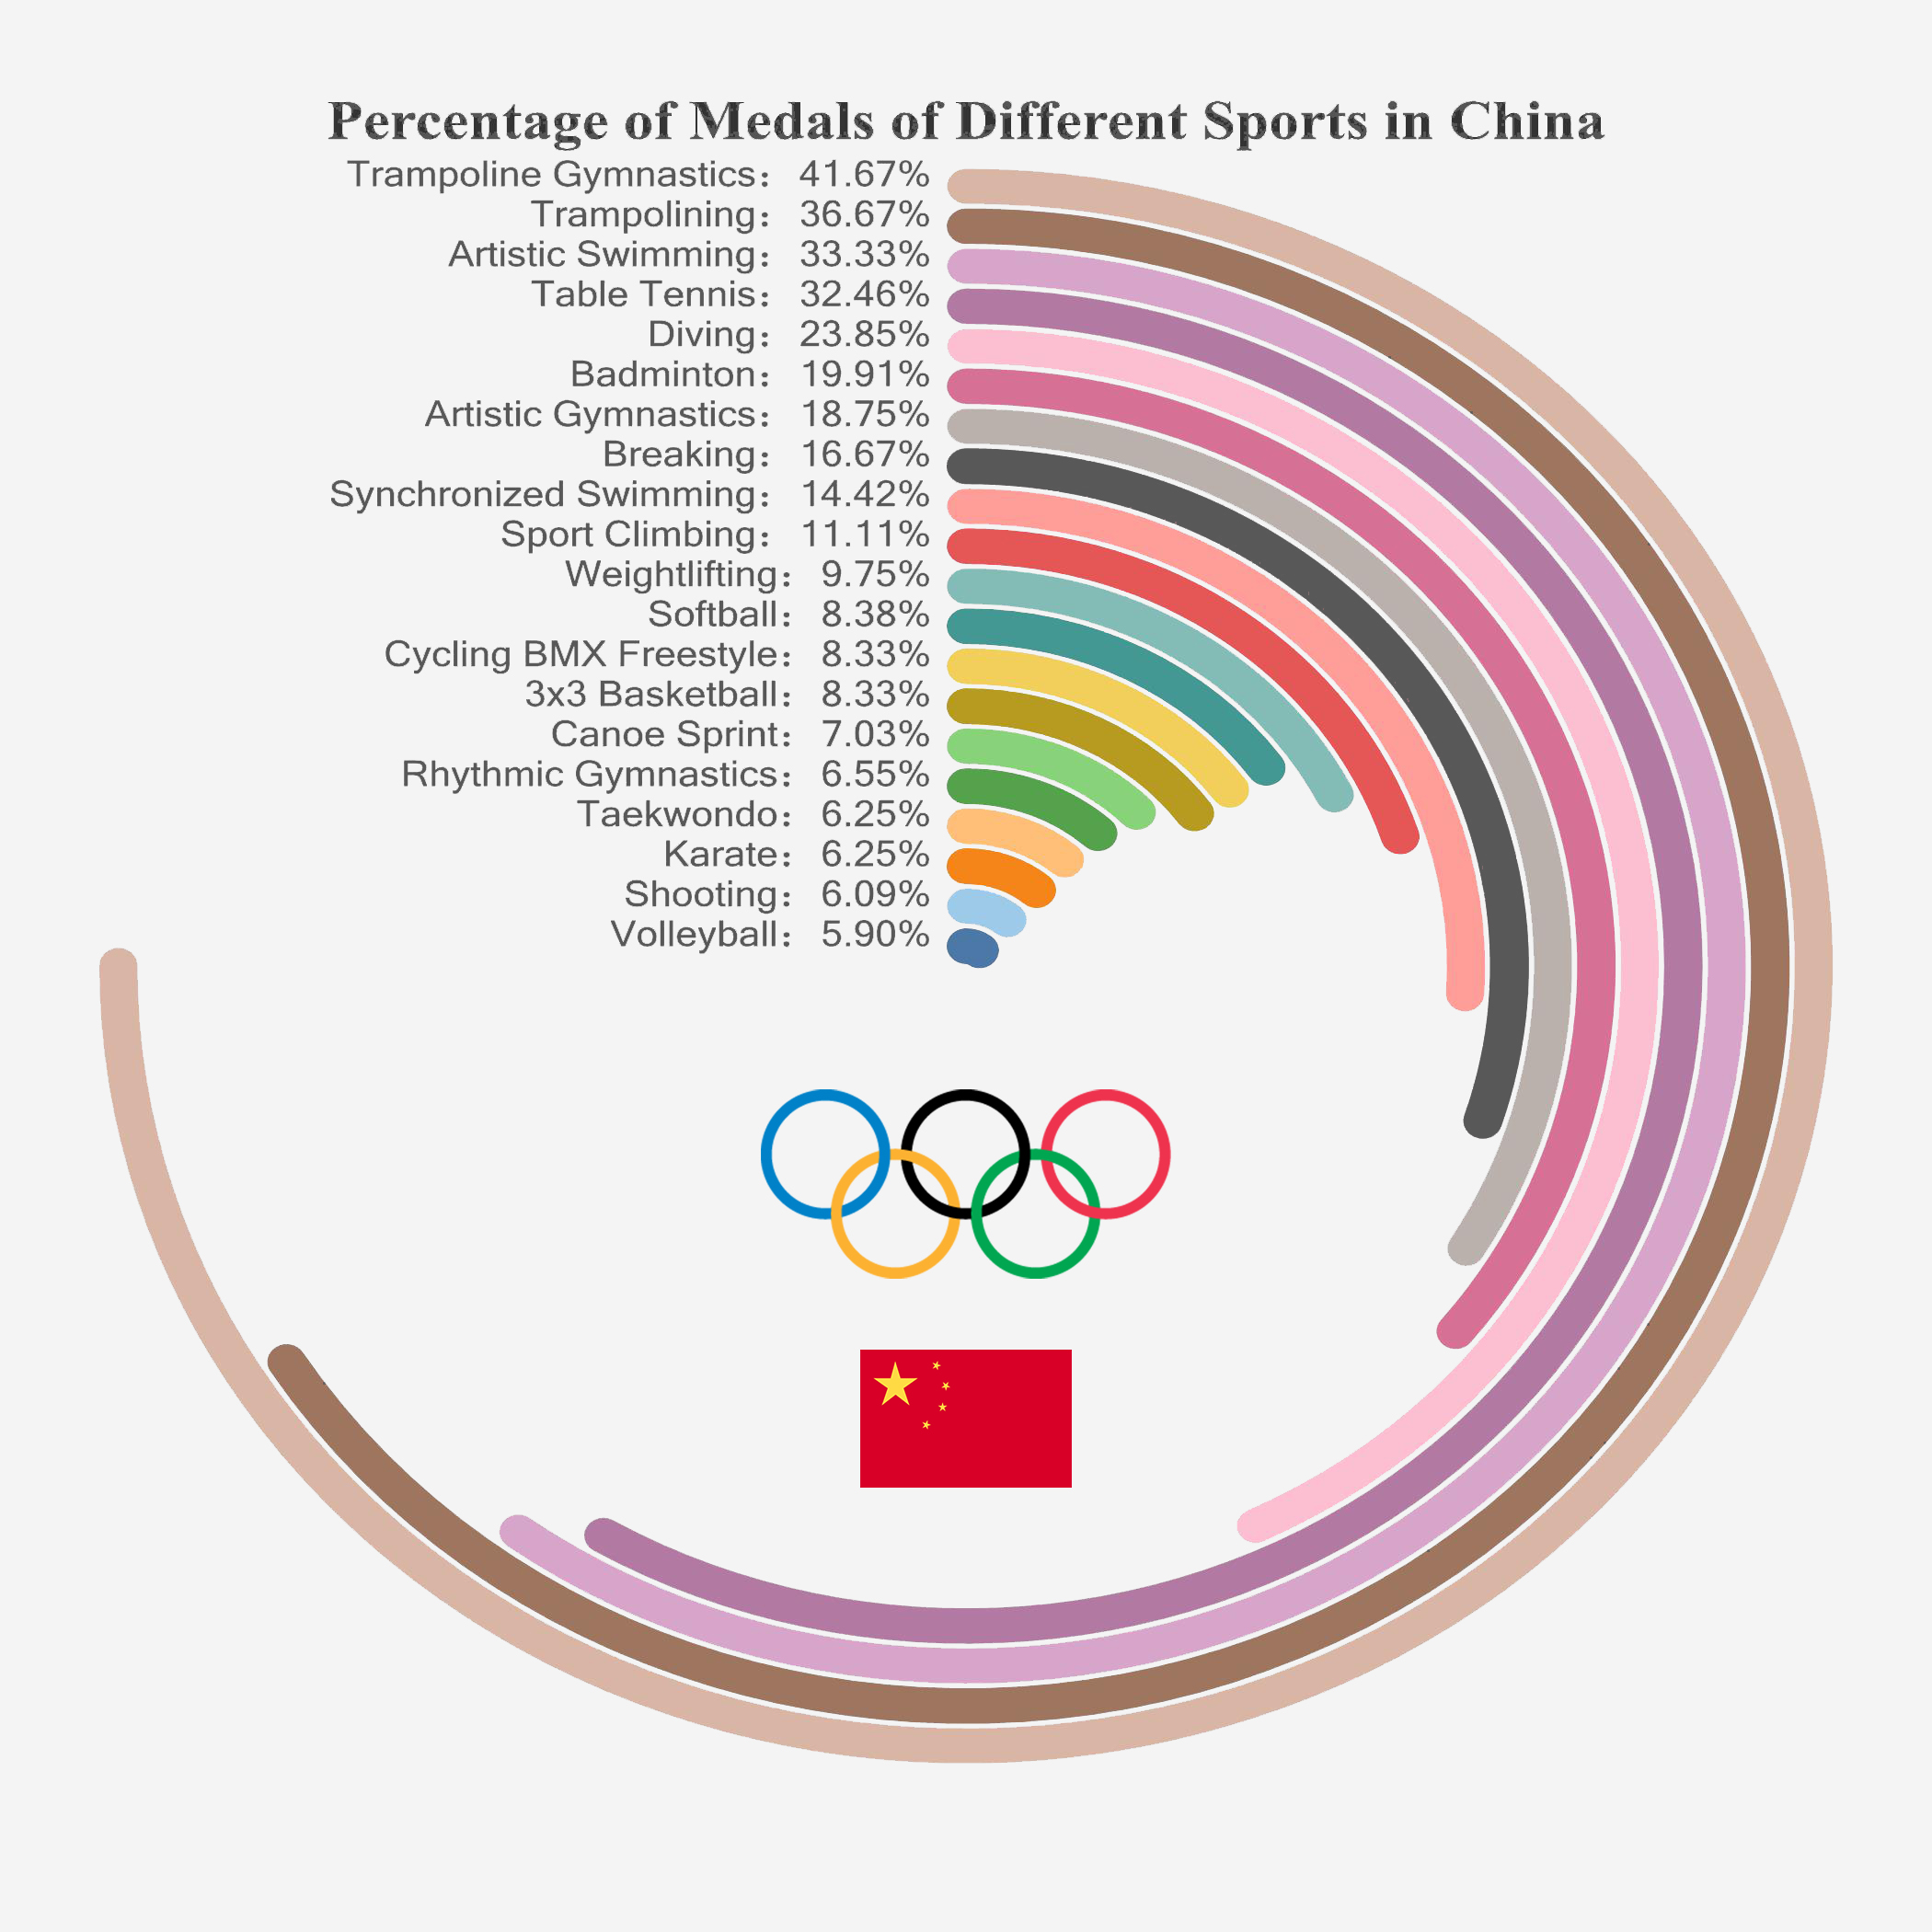
\includegraphics[width=12cm]{img/Percentage.jpg}
	\caption{Percentage of Medals of Different Sports in China}
	\label{fig:aa}
\end{figure}






\section{Task1:Medal Prediction Model Based on LightGBM}
\subsection{Medal Standings}
The detail can be described by equation \eqref{eq1}:\autoref{eq1}:
%带标签的方程
\begin{equation}\label{eq1}
\alpha+\beta=\gamma
\end{equation}
%不带标签的方程
\[
\alpha+\beta=\gamma
\]
$$\alpha$$


\[
\gamma = \frac{m_{c_i s_j}}{\sum m_{c_i s_j}}
\]

%长等式
\begin{equation}\label{eq2}
	\begin{split}
	&A+B+C+D+E+F\\
	&=G+Q+W+E+R+T+Y\\
	&=A+S+D+F+G+H+J
	\end{split}
\end{equation}
%分段方程
\begin{equation}\label{eq3}
	F(x)=
	\begin{cases}
		0&,\text{if $x<0$}\\
		x+1&,\text{if $x>0$}\\
		1&,\text{otherwise}
			\end{cases}
\end{equation}

%Table 2 : Variable Name
\begin{longtblr}[
	caption = {Variable Name},
	]{
		vline{1-4} = {1-10}{},
		hline{1-11} = {1-3}{},
	}
	Variable Name                                                    & \textit{Code}                                                & Definition                                                                      &  \\
	Whether~Host Country                                             & \textit{is host}                                             & {Whether the country is the host(1 for host,0 for\\~non-host)}                  &  \\
	{Medal Expectation\\Increment *Personnel\\Expectation lncrement} & {\textit{medal\_increment *}\\\textit{personnel\_increment}} & {Product of medal\\expectation increment and\\personnel expectation\\increment} &  \\
	{Sport Advantage\\Coefficient}                                 & \textit{sport\_adv}                                           & {Advantage coefficient of\\a specific sport}                                  &  \\
	Country Level                                                    & \textit{country\_lvl}                                        & {The level of the country in the competition\\(ordered by rank)}                &  \\
	{Project Medal\\Expectation /Project\\Personnel Expection~}                         & \textit{sport\_medal \_per\_ person}                          & {Ratio of sport medals to projected personnel\\for a specific sport}          &  \\
	Gold Medal Probability                                           & \textit{gold\_prob}                                          & {Probability of an athlete~\\winning a gold medal}                              &  \\
	{Silver Medal\\Probability}                                      & \textit{silver\_prob}                                        & Probability of an athlete~ winning a silver medal                               &  \\
	{Bronze Medal\\Probability}                                      & \textit{silver\_prob}                                        & Probability of an athletewinning a bronze medal                                 &  \\
	No Medal Probability                                             & \textit{no\_medal\_probe}                                    & Probability of an athlete winning no medal                                      &  \\
	&                                                              &                                                                                 &  \\
	&                                                              &                                                                                 &  
\end{longtblr}



%奖牌榜预测图

\begin{figure}[htbp]
	\centering
	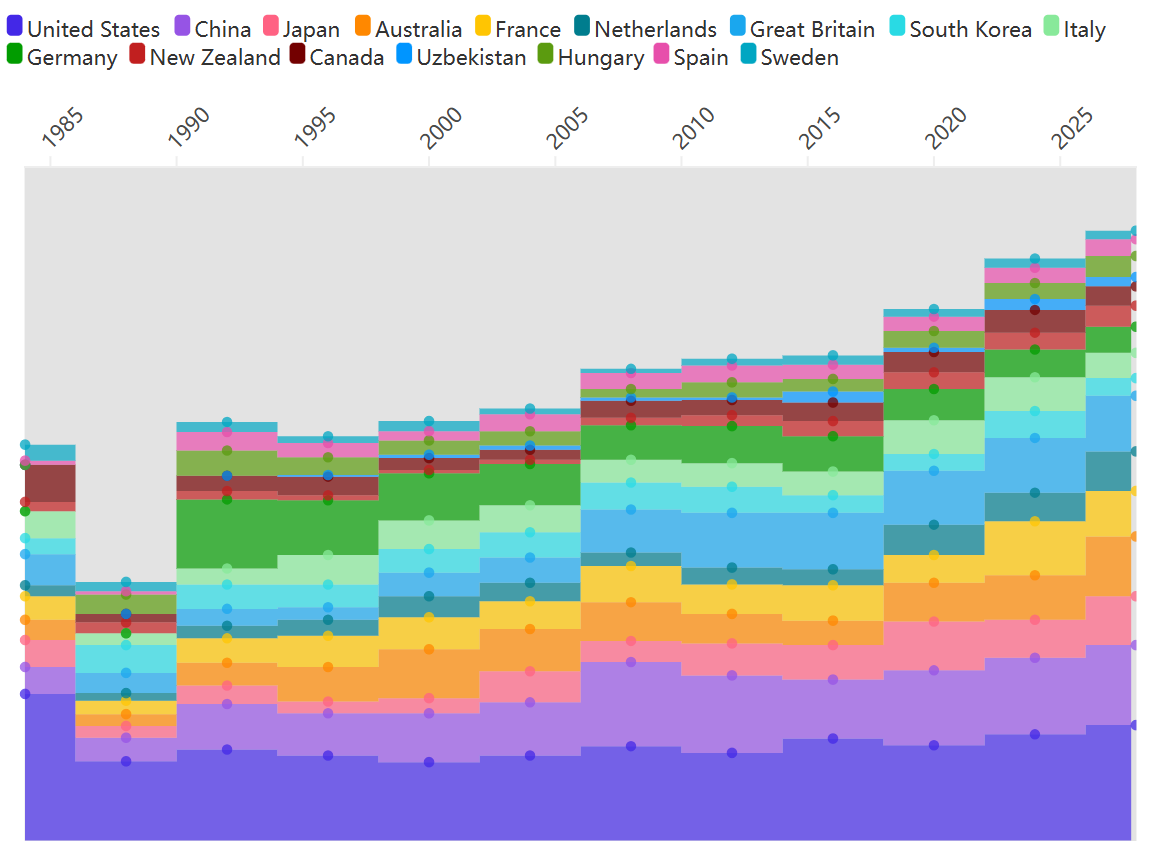
\includegraphics[width=12cm]{img/Predict.png}
	\caption{Medal count prediction}
	\label{fig:aa}
\end{figure}

\subsection{Countries that Win Their First Medal}

%首奖可能性图

\begin{figure}[htbp]
	\centering
	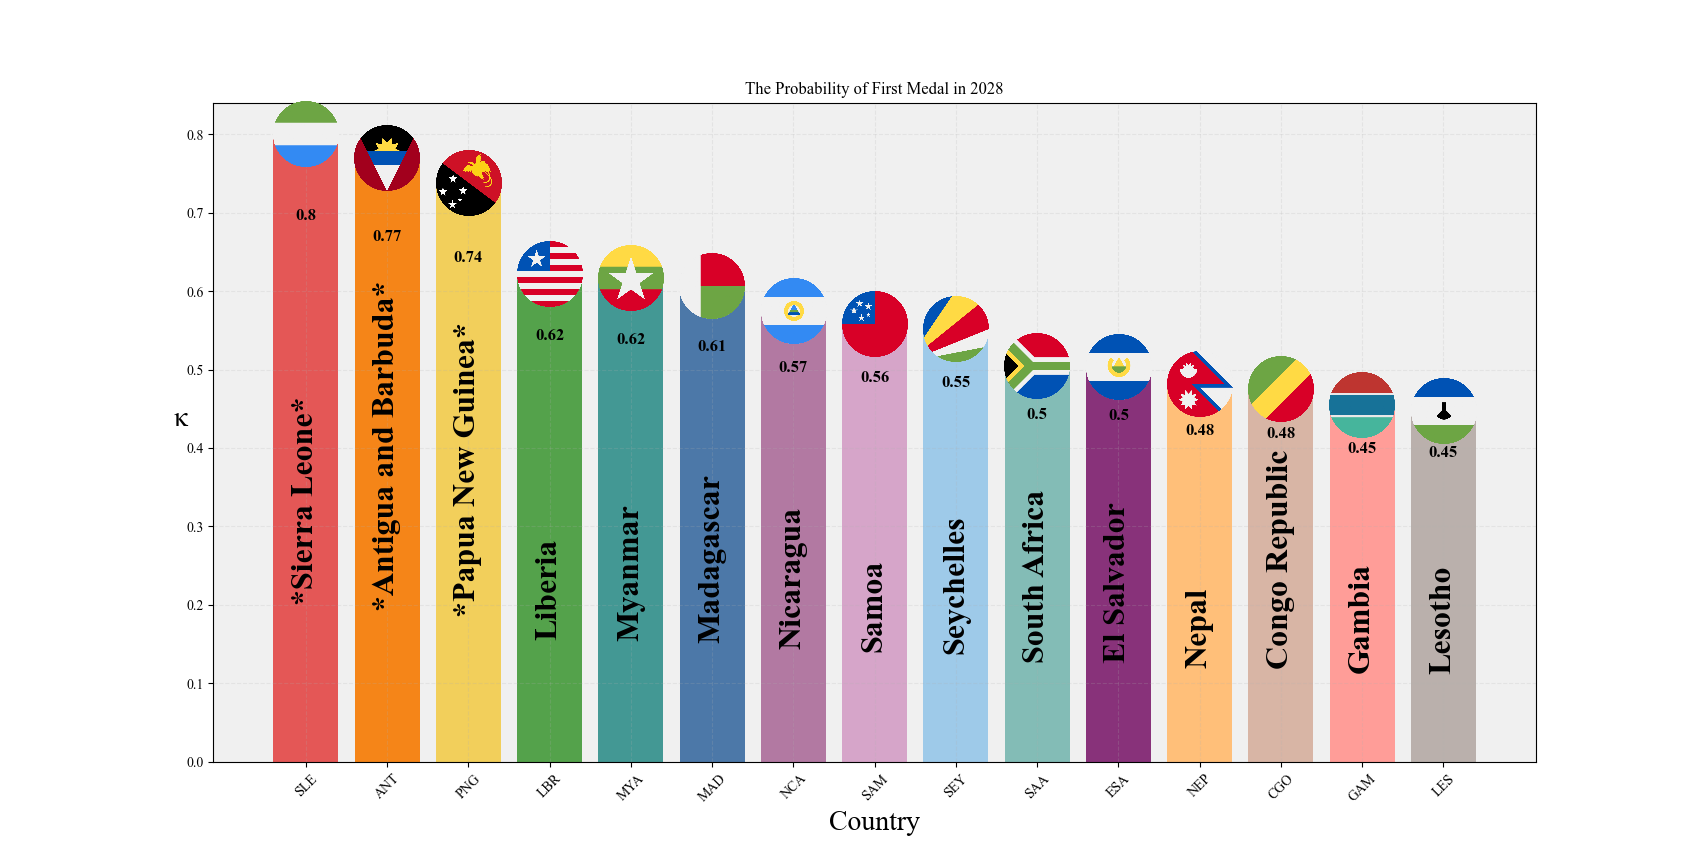
\includegraphics[width=16cm]{img/First.png}
	\caption{The Probability of First Medal in 2028}
	\label{fig:aa}
\end{figure}




\subsection{Events and Medal Counts by Countries}





%三个国家擅长项目的图
\begin{figure}[htbp]
	\centering
	\begin{subfigure}[b]{.3\textwidth}
		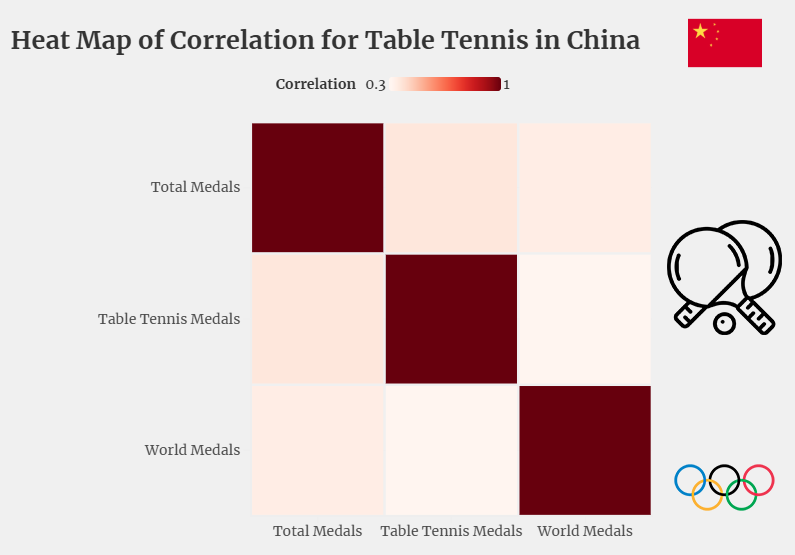
\includegraphics[width=\textwidth]{img/Table Tennis.png}
		\caption{Heatmap of Correlation for Table Tennis in China}\label{subfig:1}
	\end{subfigure}
	\hfill 
	\begin{subfigure}[b]{.33\textwidth}
		
\includegraphics[width=\textwidth]{img/Jamaica.png}
		\caption{ Heatmap of Correlation for Athletics in Jamaica}\label{subfig:2}
	\end{subfigure}
	\hfill 
	\begin{subfigure}[b]{.32\textwidth}
		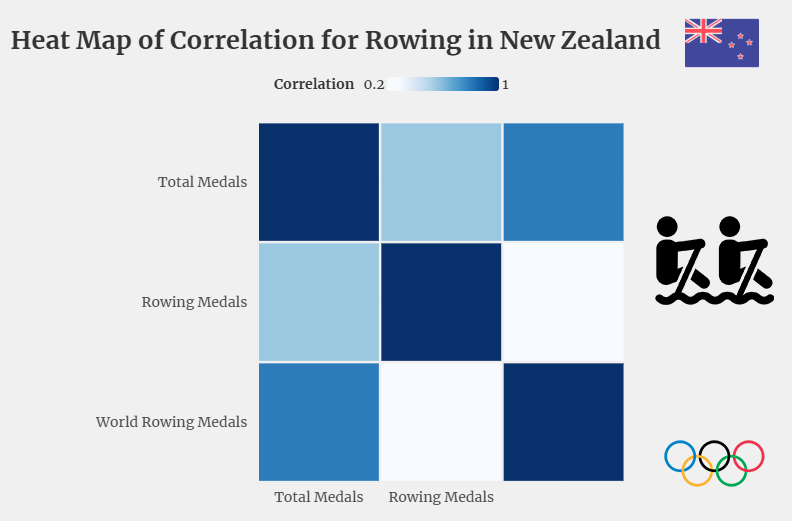
\includegraphics[width=\textwidth]{img/New Zealand.png}
		\caption{Heatmap of Correlation for Rowing in New Zealand}\label{subfig:3}
	\end{subfigure}
	\caption{Three images}\label{fig:subfigures}
\end{figure}



\section{Task2:}

The results are shown in Figure \ref{fig:result}, where $t$ denotes the time in seconds, and $c$ refers to the concentration of water in the boiler.


\clearpage







%引用图像示例Figure \ref{fig:subfigures}
%Figure \ref{fig:subfigures} gives an example of subfigures. Figure \ref{subfig:left} is on the left, and Figure \ref{subfig:right} is on the right.



% \usepackage{longtable}

\begin{longtable}{l|l|l|l|l} 
	\caption{Model Performances(LightGBM)}\\ 
	\hline
	\multicolumn{1}{c|}{\textbf{Model}} & \multicolumn{1}{c|}{\textbf{MSE}} & \multicolumn{1}{c|}{\textbf{RMSE}} & \multicolumn{1}{c|}{\textbf{MAE}} & \multicolumn{1}{c}{\(\mathbf{R}^2\)}  \endfirsthead 
	\hline
	Gold Prediction                     & 0.0235                            & 0.180                              & 0.030                             & 0.690                              \\ 
	\hline
	Silver Prediction                   & 0.0239                            & 0.185                              & 0.033                             & 0.625                              \\ 
	\hline
	Bronze Prediction                   & 0.0231                            & 0.187                              & 0.034                             & 0.606                              \\
	\hline
\end{longtable}





\begin{figure}[htbp]
	\centering
	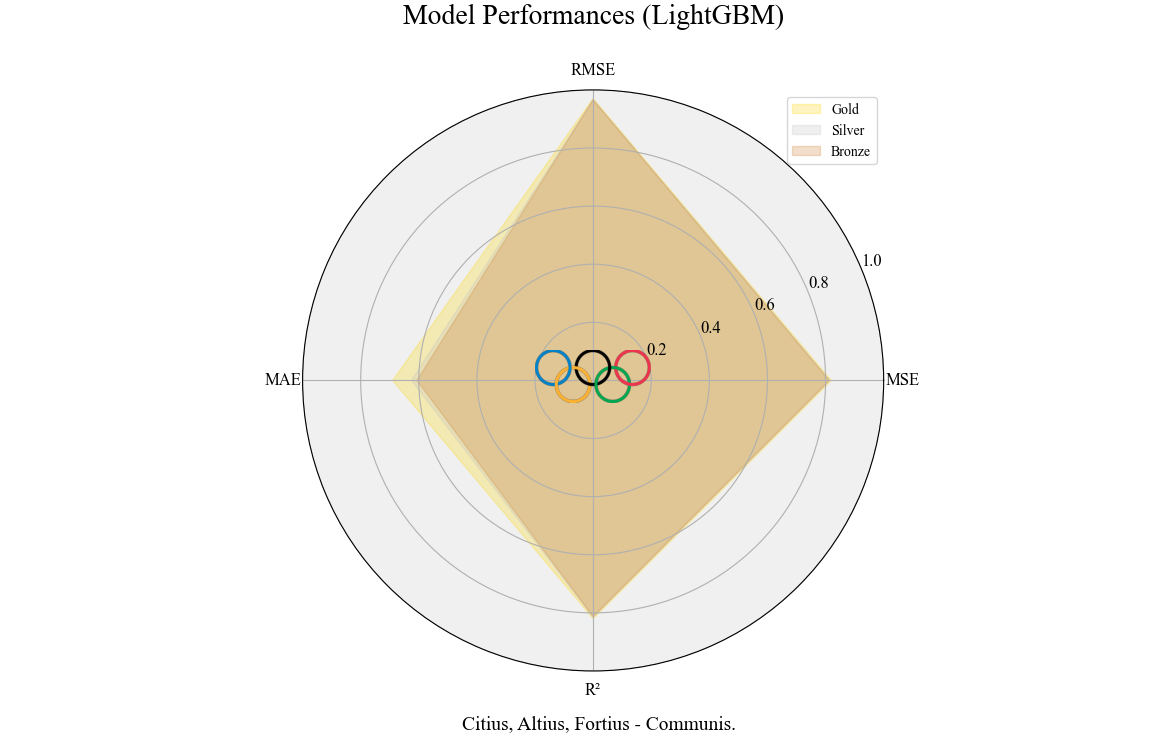
\includegraphics[width=16cm]{img/Performance.png}
	\caption{Model Performance Radar Chart}
	\label{fig:aa}
\end{figure}








\section{Task3}

%公式代码集合

\[
\mathcal{L} = \sum_{i=1}^{n} L(y_i, \hat{y}_i^{(m-1)} + \eta f_m(x_i)) + \Omega(f_m)
\]


$y_i$\\
$\hat{y}_i^{(m-1)}$\\
$\eta f_m(x_i)$\\
$\Omega(f_m)$\\




\[
\kappa = 0.8 \times \frac{\xi - \overline{\xi}}{\sigma}
\]
$\overline{\xi}$
$\sigma$


\[
d_i = R(X_i) - R(Y_i)
\]
\[
R_s = 1 - \frac{6 \sum d_i^2}{n(n^2 - 1)}
\]
$d_i$
$R_s$


\[
P(c_k \mid X) = \frac{P(X \mid c_k) P(c_k)}{P(X)}
\]

\[
	C_t^+ = \max(0, C_{t-1}^+ + (X_t - \mu - k))
\]
\section{Task4}













\section{Sensitivity Analysis}

\section{Model Evaluation}
\subsection{Strengths}
\begin{itemize}
    \item First one...
    \item Second one ...
\end{itemize}

\subsection{Weaknesses}
\begin{itemize}
    \item Only one ...
 \end{itemize}
 
\section{Conclusion}

% 以下为信件/备忘录部分,不需要可自行去掉
% 如有需要可将整个 letter 环境移动到文章开头或中间
% 请在第二个花括号内填写标题,如「信件」(Letter)或「备忘录」(Memorandum)
\begin{letter}{Memorandum}
\begin{flushleft}  % 左对齐环境,无首行缩进
\textbf{To:} Heishan Yan\\
\textbf{From:} Team 1234567\\
\textbf{Date:} October 1st, 2019\\
\textbf{Subject:} A better choice than MS Word: \LaTeX
\end{flushleft}

In the memo, we want to introduce you an alternate typesetting program to the prevailing MS Word: \textbf{\LaTeX}. In fact, the history of \LaTeX\ is even longer than that of MS Word. In 1970s, the famous computer scientist Donald Knuth first came out with a typesetting program, which named \TeX\ \ldots

Firstly, \ldots

Secondly, \ldots

Lastly, \ldots

According to all those mentioned above, it is really worth to have a try on \LaTeX! 
\end{letter}


% 参考文献,此处以 MLA 引用格式为例
\begin{thebibliography}{99}
\bibitem{1} Einstein, A., Podolsky, B., \& Rosen, N. (1935). Can quantum-mechanical description of physical reality be considered complete?. \emph{Physical review}, 47(10), 777.
\bibitem{2} \emph{A simple, easy \LaTeX\ template for MCM/ICM: EasyMCM}. (2018). Retrieved December 1, 2019, from\url{https://www.cnblogs.com/xjtu-blacksmith/p/easymcm.html}
\end{thebibliography}


% 以下为附录内容
% 如您的论文中不需要附录,请自行删除
\begin{subappendices}  % 附录环境

\section{Appendix A: Further on \LaTeX}
To clarify the importance of using \LaTeX\ in MCM or ICM, several points need to be covered, which are \ldots

To be more specific, \ldots

All in all, \ldots

Anyway, nobody \textbf{really} needs such appendix \ldots

\section{Appendix B: Program Codes}
Here are the program codes we used in our research.

% 代码环境示例三则
% 如您的论文不需要展示代码,请删除
% 更多用法,请参考 listings 宏包文档

% Python 代码示例
\begin{lstlisting}[language=Python, name={test.py}]
# Python code example
for i in range(10):
    print('Hello, world!')
\end{lstlisting}

% MATLAB 代码示例
\begin{lstlisting}[language=MATLAB, name={test.m}]
% MATLAB code example
for i = 1:10
    disp("hello, world!");
end
\end{lstlisting}



% C++ 代码示例
\begin{lstlisting}[language=C++, name={test.cpp}]
// C++ code example
#include <iostream>
using namespace std;

int main() {
    for (int i = 0; i < 10; i++)
        cout << "hello, world" << endl;
    return 0;
}
\end{lstlisting}

\end{subappendices}  % 附录内容结束

\end{document}  % 结束
